\documentclass[10pt]{article}

\usepackage{graphicx}
\usepackage{graphics}
\usepackage{multicol}
\usepackage{epsfig,amsmath,amsfonts}

\makeatletter                                   % Make '@' accessible. 
\oddsidemargin=0in                              % Left margin minus 1 inch.
\evensidemargin=0in                             % Same for even-numbered pages.
\marginparsep=0pt                               % Space between margin & text

\renewcommand{\baselinestretch}{1}              % Double spacing

\textwidth=6.5in                                % Text width (8.5in - margins).
\textheight=9in                                 % Body height (incl. footnotes)

\topmargin=0in                                  % Top margin minus 1 inch.
\headsep=0.0in                                  % Distance from header to body.
\skip\footins=4ex                               % Space above first footnote.
\hbadness=10000                                 % No "underfull hbox" messages.
\makeatother                                    % Make '@' special again.


\begin{document}

\fontfamily{cmss}                               % Make text sans serif.
\fontseries{m}                                  % Medium spacing.
\fontshape{n}                                   % Normal: not bold, etc.
\fontsize{10}{10}                               % 10pt font, 10pt line spacing 

\title{Ad-Hoc Routing Component Architecture}
\author{Philip Levis et al.}
\maketitle

\fontfamily{cmr}                                % Make text Roman (serif).
\fontseries{m}                                  % Medium spacing.
\fontshape{n}                                   % Normal: not bold, etc.
\fontsize{10}{10}                               % 10pt font, 10pt line spacing


\begin{figure}
\centering
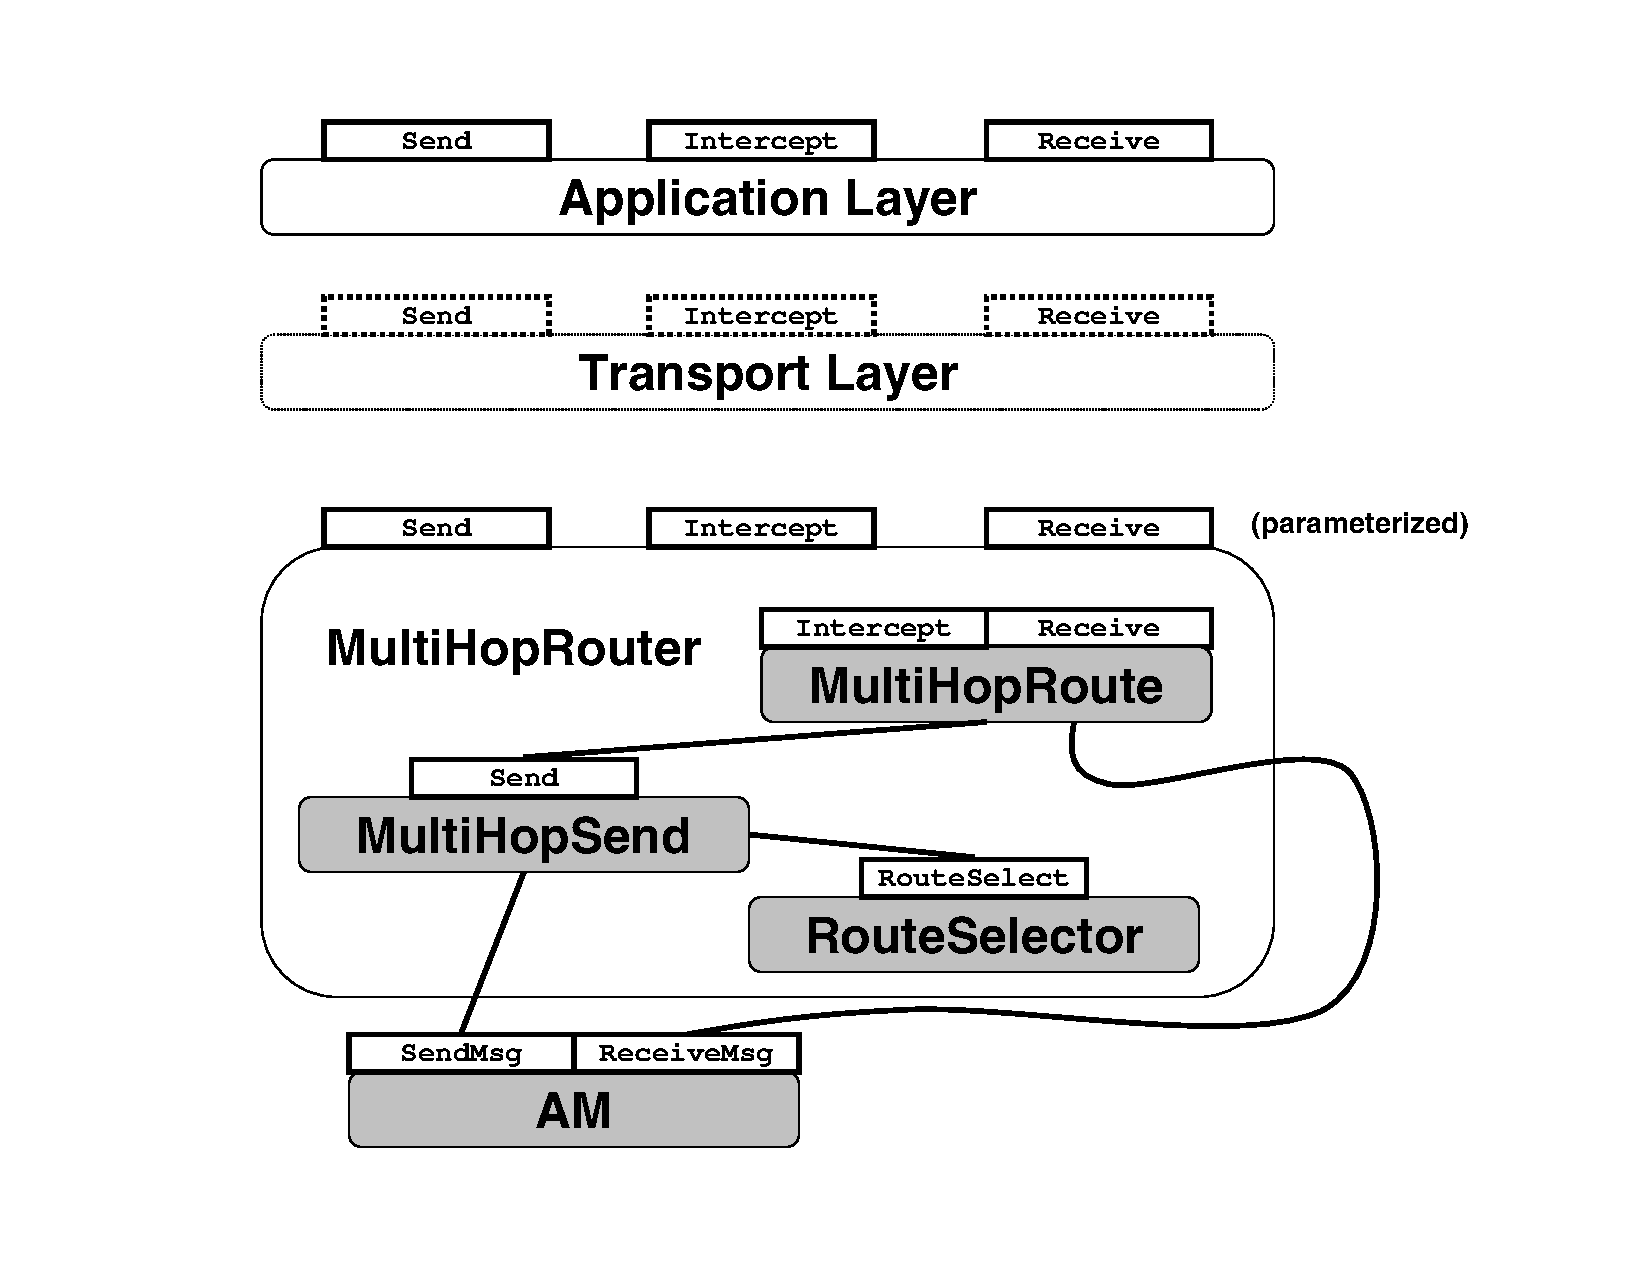
\includegraphics[angle=-90,scale=.25]{fig/arch.pdf}
\caption{Component Architecture}
\label{fig:arch}
\end{figure}


\section*{Introduction}

TinyOS has a pressing need for a good ad-hoc routing service. Several
protocols have been developed, each of which has acknowledged
problems. One issue that has arisen is separating policies from
mechanisms; it would be a great help to have the ability to easily
experiment with a variety of different algorithmic building blocks,
each of which can be easily interchanged. We have therefore developed
a general ad-hoc protocol component architecture; algorithms should be
built in components that follow this architecture, so that they can be
easily incorporated into different combinations for testing and
evaluation.

\section*{Overview}

Multi-hop routing has been broken into several components, shown in
Figure \ref{fig:arch}. At the top of the architecture is an
application component. Between it and the multi-hop component are an
arbitrary number of networking stack components (in the diagram, this
is represented by a possible Transport component). An application
interacts with the network stack through the {\tt Send} and {\tt
Receive} interfaces; use of the {\tt Intercept} interface is optional,
for in-network processing.

MultiHopRouter is the top-level configuration for the routing layer;
higher protocol layers interact with the subsystem through
MultiHopRouter's provided interfaces.

\subsection*{Sending a Packet}

Before sending a packet, a component should use the {\tt getBuffer}
command to obtain a pointer to the data region of a packet. This call
allows interface users to remain unaware of the packet format used by
the provider. Calling the {\tt Send} interface's {\tt getBuffer} has
the side effect of initializing protocol fields to denote that the
current mote is the source of the packet. In the case of end-to-end
protocols, such as ad-hoc routing, only the originator of the packet
should call {\tt Send.getBuffer}.

Calling {\tt Send.send} on MultiHopRouter calls MultiHopSend's {\tt
send} command. MultiHopSend calls the MultiHopRoute component, which
chooses a route and fills in the appropriate fields. Once the route
has been selected, the packet can then be transmitted through the AM
{\tt SendMsg} interface.

MultiHopRoute depends on some number of Estimator components to make
decisions on which route to use (not shown). For example, a min-hop
algorithm (similar to BLESS or Narpro) might have an estimator that
listens for protocol messages and updates routing tables
accordingly. A network link quality estimator might use link quality
broadcasts to communicate with neighbors. A given RouteSelector uses
some set of Estimators, each of which can have its own specific
interface, to decide on a route.

\subsection*{Routing/Receiving a Packet}

AM's message reception signals MultiHopRoute.  MultiHopRoute
determines if the packet is destined for the local node. If so, it
signals MultiHopRouter's {\tt Receive} interface.

If not, it signals MultiHopRouter's {\tt Intercept} interface, which
allows higher-level components to peek into and modify packet
payloads. The return code on the {\tt Intercept} event states whether
the multi-hop layer should send the packet or not; components can
aggregate data from several packets using this mechanism. The default
{\tt Intercept} handler forwards all packets.

To forward the packet, MultiHopRoute calls {\tt Send.send} on
MultiHopSend, using the same sending policy as if it was the packet
originator.

\subsection*{Naming}

This ad-hoc routing architecture does not deal with the issue of
naming; it is designed for a collection routing scheme, in which many
nodes send to a single root. Naming could, however, be incorporated by
adding additional naming interfaces; for example, MultiHopRouter could
have an interface that fills in a network name given a geographical
location.

\section*{Roles}

\subsubsection*{MultiHopSend}

MultiHopSend is responsible for sending packets using the implemented
ad-hoc routing protocol. When a packet originates at a node (as
opposed to being forwarded), the application must call {\tt
getBuffer()} before calling {\tt send()}. This allows MultiHopSend to
set protocol fields to unique values so that it can distinguish
forwarded from originated packets (this can be important in the
presence of originator fields, etc.). MultiHopSend accomplishes this
by calling {\tt RouteSelect.initializeFields} on RouteSelector.

MultiHopSend does not have any route selection logic and does not fill
in the header fields necessary to send a packet; this is all performed
by RouteSelector. It is, however, responsible for decisions such as
when and how many times to retransmit, and when alternate parents
should be requested.

\subsubsection*{MultiHopRoute}

MultiHopRoute is responsible for receiving protocol messages and
deciding whether it should forward them. If MultiHopRoute decides that
it should forward a message, then it passes the packet to MultiHopSend.

\subsubsection*{RouteSelector}

RouteSelector maintains routing state, which it uses to choose routes
for packets to send. MultiHopSend passes it a packet buffer, which it
fills in with the necessary header fields to be later understood by
MultiHopRoute. RouteSelector makes its routing decisions using some
number of Estimators, each of which can have different interfaces. For
example, there might be a LinkQualityEstimator, a
GeographicPositionEstimator, and a PowerEstimator, the combination of
which are used to choose power-minimizing high-quality links that make
geographic progress to the desired destination.


\section*{Interfaces}

\subsection*{Send.nc}
\scriptsize
\begin{verbatim}
/*
 * Authors:		Philip Levis
 * Date last modified:  8/12/02
 *
 * The Send interface should be provided by all protocols above layer
 * 2 (GenericComm/AM). For example, ad-hoc routing protocols should
 * provide this interface for sending packets.
 *
 * The goal of this interface is to allow applications to take part in
 * buffer swapping (avoiding the mbuf problem) on send while being
 * unaware of the structure of the underlying packet. When an
 * application wants to send a packet, it should call getBuffer(),
 * passing the packet buffer it will use. The underlying component,
 * aware of the structure of its headers and footers, returns a
 * pointer to the area of the packet that the application can fill
 * with data; it also provides the length of the usable region within
 * the buffer.
 *
 * The application can then fill this region with data and send it with
 * the send() call, stating how much of the region was used.
 *
 * getBuffer(), when called, should set all protocol fields into a
 * unique and recognizable state. This way, when a buffer is passed to
 * send(), the component can distinguish between packets that are
 * being forwarded and those that are originating at the mote.
 * Therefore, getBuffer() should not be called on a packet that is
 * being forwarded.
 *
 */

includes AM;
interface Send { 
  command result_t send(TOS_MsgPtr msg, uint16_t length);
  command uint8_t* getBuffer(TOS_MsgPtr msg, uint16_t* length);
  event result_t sendDone(TOS_MsgPtr msg, result_t success);
}
\end{verbatim}
\normalsize


\subsection*{Receive.nc}
\scriptsize
\begin{verbatim}
/*
 * Authors:             Philip Levis
 * Date last modified:  1/30/03
 *
 * The Receive interface should be provided by all protocols above layer
 * 2 (GenericComm/AM). For example, ad-hoc routing protocols should
 * provide this interface for receiving packets.
 *
 * The goal of this interface is to allow network end-points to
 * receive packet payloads without having to know about the internal
 * structure of the packet or the layers below them in the stack.
 *
 * The Receive interface is only used at the communication end-point,
 * allowing a buffer swap between the top-level application and the
 * networking stack. Hops along the way that want to look at the
 * internals of the packet (for in-network aggregation, for example),
 * should use the Intercept interface.
 *
 * For example, if a packet takes the route A->B->C->D
 *
 * A: send();
 * B: intercept();
 * C: intercept();
 * D: receive();
 */

includes AM;
interface Receive {
  event TOS_MsgPtr receive(TOS_MsgPtr msg, void* payload, uint8_t payloadLen);
  
}

\end{verbatim}
\normalsize

\subsection*{Intercept.nc}
\scriptsize
\begin{verbatim}
/*
 * Authors:             Philip Levis
 * Date last modified:  1/30/03
 *
 * The Intercept interface should be provided by all protocols above layer
 * 2 (GenericComm/AM). For example, ad-hoc routing protocols should
 * provide this interface for in-network packet processing.
 *
 * The goal of this interface is to allow transmission hops to
 * process packet payloads without having to know about the internal
 * structure of the packet or the layers below them in the stack.
 *
 * The Interface interface is only used by nodes that are forwarding a
 * multihop messages. A protocol layer does not perform a buffer swap, but
 * can tell lower layers to not forward a packet by giving a FAIL return value.
 * Using this, an in-network intermediary can receive multiple packets,
 * aggregate their results, then forward them on to the destination.
 *
 * For example, if a packet takes the route A->B->C->D
 *
 * A: send();
 * B: intercept();
 * C: intercept();
 * D: receive();
 */

includes AM;
interface Intercept {
  /**
   *
   * Signals that a message has been received, which is supposed to be
   * forwarded to another destination. Allows protocol layers above the
   * routing layer to perform data aggregation or make application-specific
   * decisions on whether to forward.
   *
   * @param msg The complete buffer received.
   *
   * @param payload The payload portion of the packet for this
   * protocol layer. If this layer has layers above it, it should signal
   * receive() with payload incremented by the size of its header. Payload
   * is a pointer into the msg structure.
   *
   * @param payloadLen The length of the payload buffer. If this layer
   * has layers above it, it should signal receive() with payloadLen
   * decreased by the size of its headers and footers.
   *
   * @return SUCCESS indicates the packet should be forwarded, FAIL
   * indicates that it should not be forwarded.
   *
   */
  event result_t intercept(TOS_MsgPtr msg, void* payload, uint8_t payloadLen);

}

\end{verbatim}
\normalsize

\subsection*{RouteSelect.nc}
\scriptsize
\begin{verbatim}
/*
 * Authors:		Philip Levis
 * Date last modified:  8/12/02
 *
 * The RouteSelect interface is part of the TinyOS ad-hoc routing
 * system architecture. The component that keeps track of routing
 * information and makes route selection decisions provides this
 * interface. When a Send component wants to send a packet, it passes
 * it to RouteSelect for its routing information to be filled in. This
 * way, the Send component is entirely unaware of the routing
 * header/footer structure.
 */

includes AM;
interface RouteSelect {
  command bool isActive();
  command result_t selectRoute(TOS_MsgPtr msg);
  command result_t initializeFields(TOS_MsgPtr msg, uint8_t id)
  command uint8_t* getBuffer(TOS_MsgPtr msg, uint16_t* len);
}
\end{verbatim}
\normalsize

\end{document}
